\projectname{} simplifies the troubleshooting process by programatically localizing the root cause
of network problems along three dimensions: {\it what} network problems exist at a
particular point in time, {\it where} in the control software a problem first developed, and
{\it when} the triggering event occurred. In this section we present 
the components of \projectname{} we have designed for performing software fault localization for SDN.

\subsection{Correspondence Checking}

In simple terms, correctness of the platform can be expressed as follows:
the policy specified by the application layer should correspond to the
configuration of the physical network. We refer to any miscorrespondence
between the policy and the configuration as a {\it policy-violation}.

We leverage the virtual packet algebra pioneered in headerspace
analysis~\cite{hsa} to verify whether the application's policies are indeed
implemented correctly in the physical network. Our algorithm, correspondence
checking, provides a crisp determination of all possible packet inputs that
would not behave according to the application's policies if injected into the
network at a particular point in time. Furthermore, running correspondence
checking between intermediate layers of the SDN stack (logical view versus
physical view), allow us to identify the component(s) of
the system where policy-violations first manifest themselves.

Formally, the state of the physical network, the physical view, and the
logical view can be represented as a graph,
$G = (V, E)$. Packets are series of bits, $h \in \{0,1\}^L = H$,
where $L$ is the maximum number of bits in the header.

Upon receiving a packet,
forwarding elements apply a transformation function, potentially modifying
packets before forwarding them on\footnote{Multicast forwarding can expressed
by extending the range to sets of output tuples}:
\begin{align*}
T: (H \times E) \rightarrow (H \times E_{\emptyset})
\end{align*}

We use $`\Psi`$ to denote the collection of all transfer functions present in
the network at a particular point in time. In this model, network traversal is simply a composition of transformation
functions. For example, if a header $h$ enters the network through edge
$e$, its state after $k$ hops will be:
\begin{align*}
\Psi^k(h,e) = \Psi(\Psi(\dots \Psi(h,e)\dots))
\end{align*}

The externally visible behavior of the network can be expressed as the
transitive closure of $\Psi$:
\begin{align*}
\Omega: (H \times E_{access}) \rightarrow (H \times E_{\emptyset}) \\
\Omega(h,e) = \Psi^{\infty}(h,e)
\end{align*}
Here, $E_{access}$ denotes access links adjacent to end-hosts.
In words, $\Omega$ is a mapping between all possible input packets inserted
into the network from an end-hosts, to the final location of the packet after
traversing the network.

In SDN, it should always be the case that:
\begin{align*}
\Omega^{view} \sim \Omega^{physical}
\end{align*}
Informally, this means that any packet injected at an access link in $G^{virtual}$ should arrive at
the same final location as the corresponding (encapsulated) packet injected at the
corresponding access link in $G^{physical}$. Note that hosts are represented
in all layers, although there may not be a one-to-one mapping between the
internal vertices of $G^{virtual}$ and $G^{physical}$.

To check correspondence in SDN, we begin by taking a causally consistent
snapshot~\cite{Chandy:1985:DSD:214451.214456} of the physical network. The routing
tables of forwarding elements can then be translated into transformation functions.
Finally, we feed a symbolic packet $x^L$ to each access link of the
network.\footnote{The rules for process wildcard bits $x^n$ are defined in
the HSA paper~\cite{hsa}} The end result is a propagation graph representing all possible paths taken by a packet injected
at the access link.

The leaves of the propagation graph represent $\Omega$. We
verify correspondence in SDN by generating propagation graphs for all SDN layers,
and comparing the leaves. Any mismatch in leaves of the propagation graphs
represent policy-violations between control applications and network
configuration.

It is important to note that correspondence checking assumes that the
application's policies are correct; it only checks whether the physical
network's configuration is isomorphic with the logical view, but does not
check for additional correctness properties such as connectivity and
loop-free routing. If the user wishes to explicitly express additional
invariants, the HSA framework used by our system can
easily check for such properties.

\subsection{\SIMULATOR{}}

Correspondence checking infers all policy-violations in the network at a
particular point in time. To complete the diagnostic puzzle, troubleshooters
need two additional pieces of information. First, troubleshooters need to
identify the events (link failures, controller failures, VM migrations,
\etc{}) that triggered a particular problem. Second, in large distributed
systems, transient policy-violations due to communication delay and hardware
failures are unavoidable; troubleshooters need to be able to differentiate
persistent (pernicious) policy-violations from transient (harmless) problems
that result from normal convergence delay.

\Simulator{} is our approach to providing this information. \Simulator{} models
the network in a single process, allowing arbitrary control over hardware
failures, 
message delays and other failure modes.

\Simulator{} replays the execution of the system against
a stream of network events (\eg{}, link failures), which can be taken
either from a production trace of low level failure and topology change
events, as enabled, \eg{}, by OFRewind~\cite{ofrewind},
or can be synthetically created. Throughout the system execution, the simulator can invoke correspondence checking at any
point in time. \Simulator{} iteratively replays
the event sequences, pruning out events are not casually related to any
particular
policy-violation. In this way, \simulator{} is able to
programatically identify the `minimal causal set' of triggering events for a
given policy violation.

Figure \ref{fig:localizing} depicts this process. Suppose that the event log
consists of events $e_{1}\dots{}e_{5}$. As the system replays the trace, a 
policy-violation is found at time $t$, before $e_{5}$. The system
begins the replay at $e_{4}$, the event immediately preceding the
policy-violation. The simulator then plays the execution of the system forward
for a static time period $t_max$. If the policy-violation is detected within the window
defined by $t_max$, $e_{4}$ is added to the `causal set' for this
policy-violation. Otherwise, it is excluded. The simulator continues this
process, running previous events both in isolation and in combination, until
it has the minimum set of events that result in the policy-violation. This set
is then output to a log for the user to inspect.

\begin{figure}[t]
    %\hspace{-10pt}
    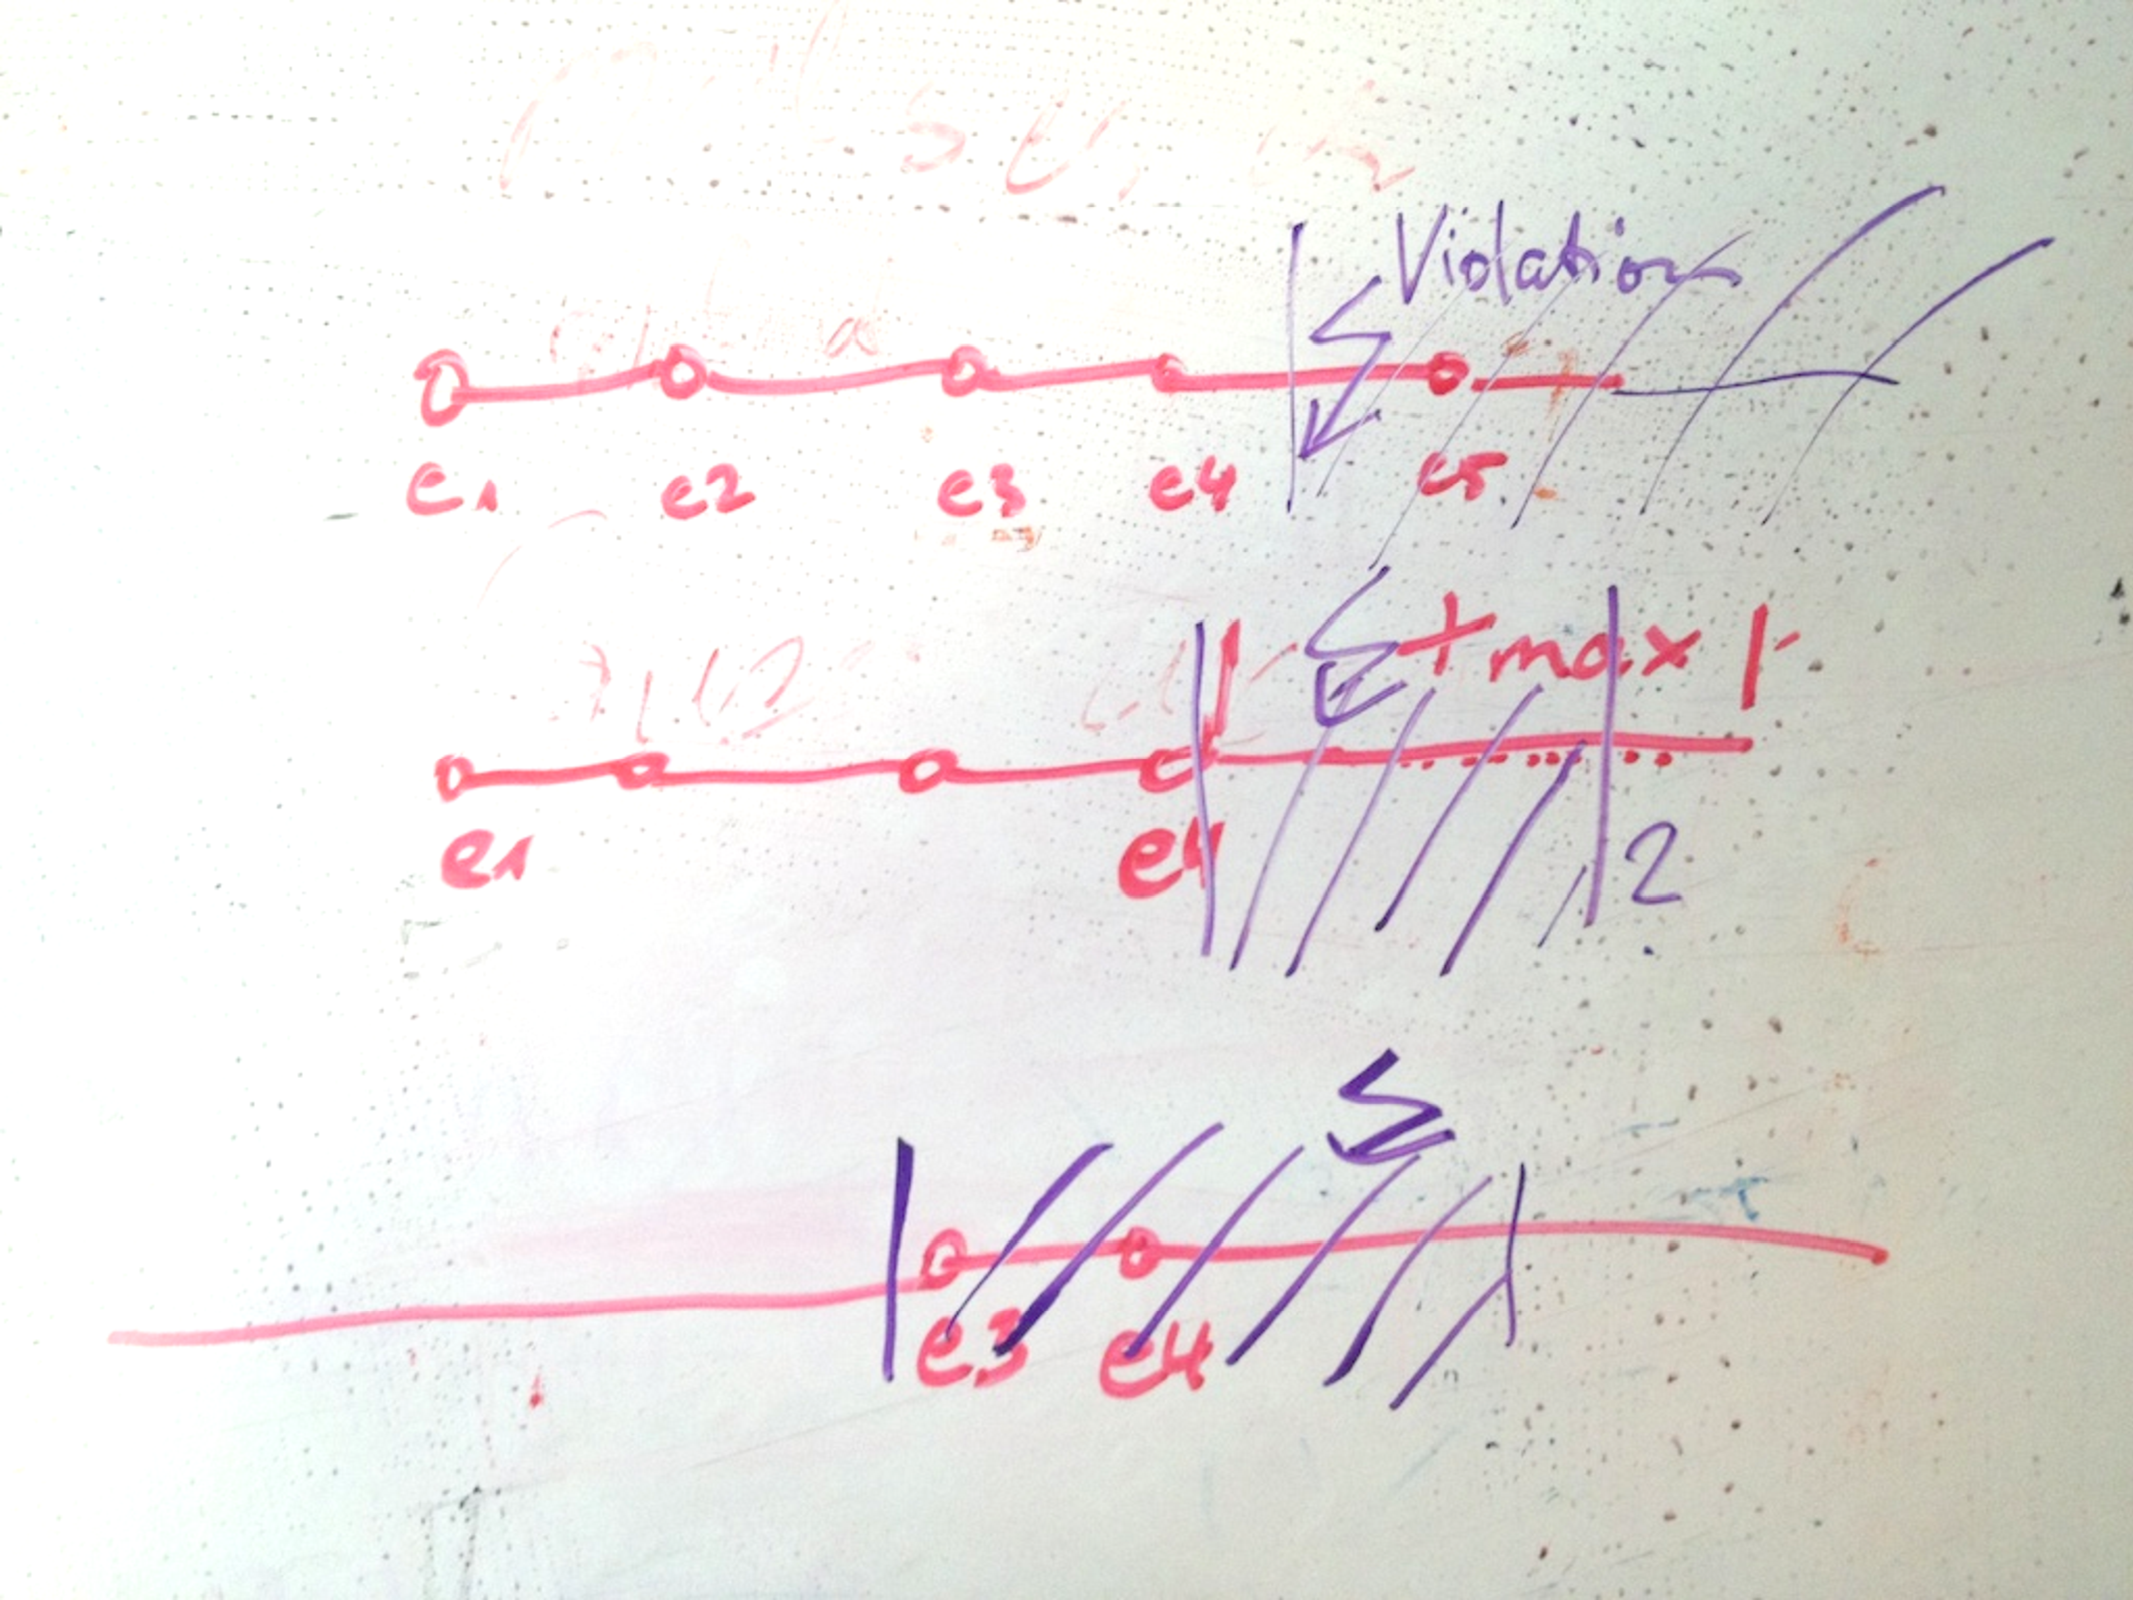
\includegraphics[width=3.25in]{../diagrams/approach/localizing}
    \caption[]{\label{fig:localizing} Localizing the minimal causal sequence for a failure in the 
    event stream}
\end{figure}

If users were to run \simulator{} on raw event logs, they would encounter a
large number of failure events and transient policy-violations. 
Replaying the system execution in a deterministic,
tightly controller environment additionally allows us
to track the life-cycle of policy-violations, effectively differentiating
transient from persistent network problems.
We describe how \simulator{} differentiates transient from persistent
policy-violations in detail below.

\textbf{Identifying persistent policy-violations}. When a policy-violation is detected,
the simulators forks off a simulation branch that investigates the future system behavior
in a case where no further external events are played out. If the detected
policy-violation
is resolved in isolation within a customizable number of simulation time steps, it is considered
a temporary problem. If it is not, this is a strong indication that the system has indeed
reached a persistent policy-violation that needs to be investigated.

\Simulator{} has a number of other possible use-cases:

\textbf{Checking related problems by fuzzing.} Input traces can be \emph{fuzzed}, i.e.,
randomly perturbed, to expose the system to similar error conditions, and confirm
that a proposed solution is not just a point-fix.

\textbf{Investigating pathological environment conditions.} The simulator allows for investigation
of pathological environment conditions difficult to achieve in a real world test bed
(\eg{}, correlated failure rates, extremely long delays etc.). This enables
investigation of situations that have a high potential for triggering errors.

\textbf{Interactive exploration.} Troubleshooters can also interactively bisect
the trace or modify specific events to further pinpoint the cause for a failure.
This is useful as soon as a suspect event sequence has been identified.

\textbf{Regression/Integration Test Library.} In traditional software engineering practices,
integration tests are an
important part of the software development cycle: developers feed end-to-end
input through the system, and verify that the system execution satisfies
certain safety and liveness properties. As additional failure cases are encountered in
production, new cases can be added to a suite of integration tests to
ensure robust operation of the system in future versions of the system.

Although the practice of accumulating an integration test suite over time is
commonplace in other fields of computer science, the field of networking
simply did not have the requisite software infrastructure to realize this practice before the emergence
of SDN. \Simulator{} can be viewed as our realization
of this development practice, applied to network controllers. Our simulator's fine-grained control over
failure scenarios allows us to test corner-case network conditions -- those
that are most difficult to anticipate in traditional unit tests.
As known failure cases are accrued over time, we envision \simulator{} being used to validate
new and existing SDN platforms. 

\subsection{Discussion}

Correspondence checking and \simulator{} serve to isolate the platform layer and
event sequence responsible for a given error. \projectname{} can be
complemented by classical debugging techniques, \eg{} log messages and source
code debugging, to identify the root cause of
the failure in the code. These techniques are much more
effective when applied a specific event sequence. Once a
potential fix has been developed, it can be validated by repeating the
problematic execution within \projectname{}. Input fuzzing further helps to
validate whether there are 
related error events that the patch missed.
